\chapter{CÁC NGHIÊN CỨU LIÊN QUAN}
\ifpdf
    \graphicspath{{Chapter2/Chapter2Figs/PNG/}{Chapter2/Chapter2Figs/PDF/}{Chapter2/Chapter2Figs/}}
\else
    \graphicspath{{Chapter2/Chapter2Figs/EPS/}{Chapter2/Chapter2Figs/}}
\fi

\markboth{\MakeUppercase{\thechapter. chapter 2}}{\thechapter. CÁC HƯỚNG TIẾP CẬN VẤN ĐỀ.}

Từ những vấn đề đặt ra ở trên, Ta có thể thấy được tính ứng dụng và ý nghĩa thực tiễn của bài toán đếm đối tượng (ví dụ như con người). Những chiến lược đã được các nhà nghiên cứu đưa ra để giải quyết bao gồm Counting by Detecion, Counting by Clustering và gần đây nhất thì phương pháp Counting by Regression đã đưa đến những kết quả đáng chú ý trong xử lý với các đam đông có mật độ lớn và phức tạp. Trong chương này. sinh viên dựa trên một công trình khảo sát thực hiện bởi Loy et al. \cite{loy2013crowd} và quá trình khảo sát của bản thân sẽ trình bày tổng quát và hệ thống hóa các phương pháp giải quyết bài toán đếm đối tượng theo ba chiến lượng nêu trên. Đặc biệt sẽ tập trung vào chiến lượng Counting by Regression, phương pháp cho thấy sự hiệu quả trong đa dạng các môi trường khác nhau.
\section{Đếm dựa trên phát hiện đối tượng}
Với vấn đề \textbf{đếm} thì hướng giải quyết dễ thấy đầu tiên và đơn giản nhất đó là phát hiện ra đối tượng và đếm nó. Mục này sẽ trình bày ngắn gọn về các phương pháp trong chiến lượng đếm dựa trên phát hiện đối tượng (Counting by Detection). \par

\textbf{Phát hiện toàn bộ (Monolithic detection):} đây là hướng tiếp cận trực quan và trực tiếp nhất đối với bài toán đếm, liệt kê số đối tượng (con người) thông qua phát hiện từng đối tượng. Quá huấn luyện cho phương pháp này sẽ tiến hành phân loại sử dụng toàn bộ các bộ phận của đối tượng trong tập dữ liệu huấn luyện (ví dụ minh họa trong hình \ref{full_detect} ). Những đặc trưng thường được sử dụng trong phương pháp này bao gồm: Haar wavelet\footnote{$https://en.wikipedia.org/wiki/Haar_wavelet$}, đặc trưng HOG(Histogram of gradient) \footnote{$https://en.wikipedia.org/wiki/Histogram_of_oriented_gradients$}, edgelet và shapelets. Việc lựa chọn sử dụng đặc trưng nào để biểu diễn cho đối tượng sẽ ảnh hưởng rất lớn đến độ chính xác và tốc độ của việc phát hiện ra đối tượng. thông thường, thì việc này sẽ đòi hỏi phải đánh đổi một trong hai, giữa sự chính xác và tốc độ. Cụ thể như phân loại phi tuyến tính như RBF Support Vector Machines (SVMs)là một phương pháp mang lại kết quả với độ chính xác cao, nhưng đổi lại thì tốc độ lạ chậm. Chính vì thế, các phương pháp phân loại tuyến tính như boosting, SVMs tuyến tính hoặc Random/Hough Forests được sử dụng phổ biến hơn. \par
\begin{figure}
  			\begin{center}
    				
    				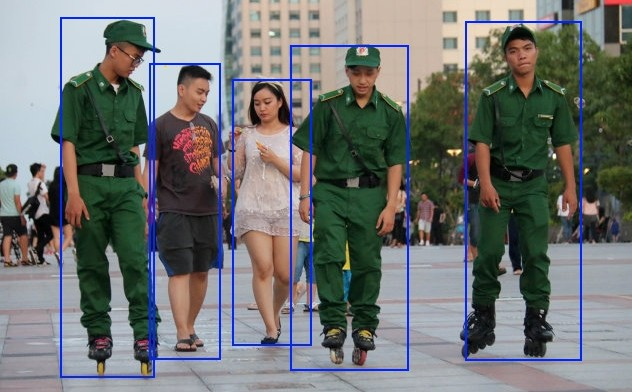
\includegraphics[scale=0.6]{full_detect}
    				\caption{phát hiện dựa trên toàn bộ đối tượng.} 
    				\label{full_detect}
  			\end{center}
\end{figure} 	
	Quá trình huấn luyện trong giai đoạn phát hiện đối tượng thường áp dụng cửa sổ trượt (sliding window) trên toàn bộ hình ảnh để tìm ra các đối tượng. Công việc này phụ thuộc nhiều và việc chọn kích thước ban đầu cho cửa sổ trượt khi mà kích thước của các đối tượng có sự chênh lệch lớn. Kèm theo đó ta sử dụng một ngưỡng độ tin cậy (thread hold) để có thể loại bỏ những vị trí có độ tin cậy thấp. Cuối cùng ta thu được tổng số lượng của các đối tượng xuất hiện trong bức hình. Việc áp dụng phát hiện dựa toàn bộ đối tượng có thể áp trong trường hợp các đối tượng xuất hiện rời rạc và rõ ràng trong hình ảnh. Tuy nhiên, đối với những trường hợp các đối tượng xuất hiện một cách lộn xộn và bị che khuất thì phương pháp này tỏ ra thiếu hiệu quả và độ chính xác thấp. \par 
	
	\textbf{Phát hiện bộ phận (Part-based detection):} như đã đề cập ở trên thì một thách thức đặt ra cho bài toán đếm đối tượng đó là việc các đối tượng bị che khuất. Để giải quyết được thách thức này, một giải pháp đã được đưa ra đó là thay vì phát hiện toàn bộ đối tượng, ta có thể chỉ cần phát hiện những bộ phận đặc trưng nhất của nó. Cụ thể hơn, đối với con người, ta có thể phân loại đó có phải là người hay không dựa vào những bộ phận đặc trưng như đầu người (ví dụ minh họa trong hình \ref{head}). Từ đó ước lượng được số lượng người xuất hiện trong hình. Người ta nhận thấy rằng, nếu chỉ sử dụng vùng đầu thì không đủ thông tin và độ tin cậy để có thể phát hiện ra đối tượng (vì có nhiều vật thể có hình dạng tương tự đầu người). Chính vì thế, mô hình phát hiện bao gồm cả đầu và vai có xu hướng mang lại kết quả tốt hơn trong thực tế. Qua đó, có thể nhận thấy so với phương pháp phát hiện toàn bộ đối tượng thì phát hiện dựa vào bộ phận sẽ giúp giảm nhẹ hơn độ phức tạp của quá trình phát hiện đối tượng và cải thiện đô chính xác trong môi trường phức tạp (có sự che khuất).
\begin{figure}
  			\begin{center}
    				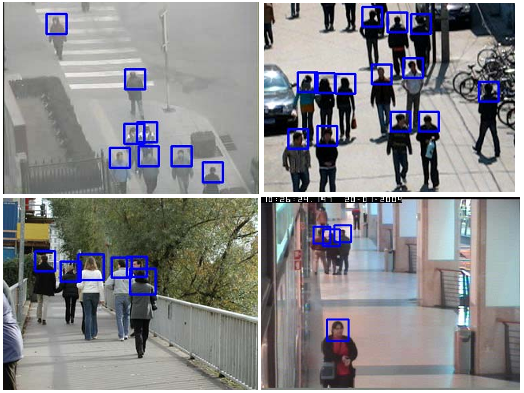
\includegraphics[scale=0.6]{head}
    				\caption{phát hiện dựa trên các bộ phận của đối tượng (đầu và vai).} 
    				\label{head}
  			\end{center}
\end{figure} 


\section{Đếm dựa trên gom cụm}
	Đếm dựa trên gom cụm (Counting by Clustering) là một hướng tiếp cận dựa trên một giả thiết được đưa ra rằng. Đối với các đối tượng riêng biệt thì thường những đặc tính như hình thức chuyển động hay các đặc điểm bên ngoài có tính tương đồng với nhau. Do đó, khi kết hợp nhằm gom nhóm quỹ đạo của những đặc tính đó với nhau có thể giúp chung ta nhận diện ra các thực thể đó. Cụ thể hơn, các nghiên cứu theo mô hình này bao gồm như \cite{Rabaud2006CountingCM}, nghiên cứu này sử dụng bộ lưu vết Kanade-Lucas-Tomasi (KLT)\footnote{$https://en.wikipedia.org/wiki/Kanade-Lucas-Tomasi_feature_tracker$} để thu được một bộ đặc tính từ bộ theo vết ở cấp thấp. Từ đó ta tập hợp quỹ đạo của các đặc tính đó rồi suy luận ra đối tượng trong bối cảnh cần xét. Cùng với đó, \cite{brostow2006unsupervised} sử dụng các đặc trưng cục bộ, sau đó sử dụng gom nhóm Bayesian\footnote{$https://www.diva-portal.org/smash/get/diva2:198852/FULLTEXT01.pdf$}
để nhóm chúng vào trong các cụm để xử lý. Một phương pháp khác liên quan chặt chẽ với chiến lượng này, \cite{tu2008unified} Đã kết hợp với ý tưởng của các đặc trưng không đổi trong mô hình Counting by Detection ở mục 2.1. Phương pháp này đầu tiên sinh ra một tập các đối tượng người dựa trên giả thuyết phát hiện đầu người. Sau đó quá trình tinh chỉnh tập trên sẽ được lặp đi lặp lại bằng cách tính toán trên các patch nhỏ trong đám đông dựa trên giả thuyết các đặc tính như các trường chuyển động, màu sắc quần áo là không thay đổi. \par

\begin{figure}%
\centering
\subfigure[]{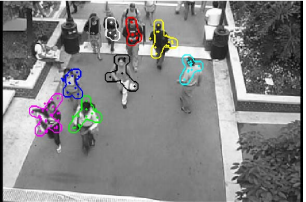
\includegraphics[width=.4\linewidth]{7}}\qquad
\subfigure[]{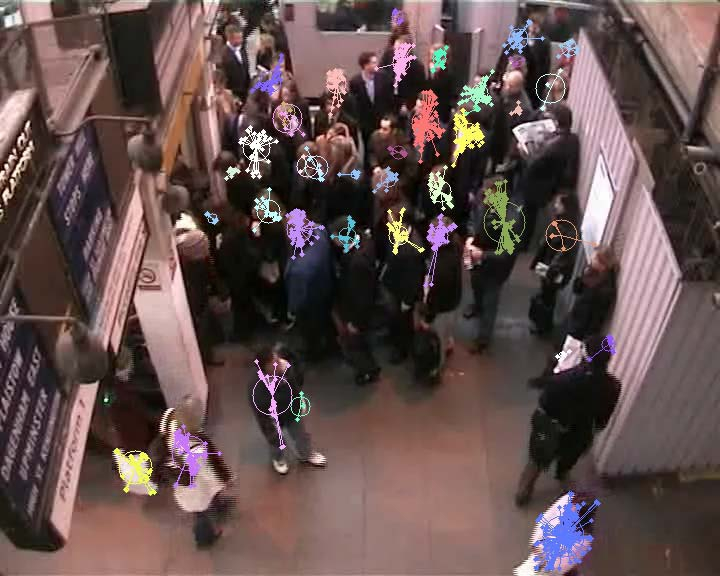
\includegraphics[width=.34\linewidth]{63}}\\
\subfigure[]{\label{3figs-c}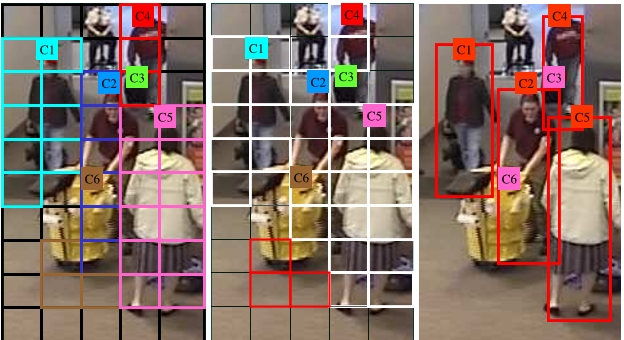
\includegraphics[width=.5\linewidth]{77}}%
\caption{(a) và (b) minh họa kết quả dựa trên việc gom nhóm các chuyển động liên kết với nhau. (c)  }
\label{3figs}
\end{figure}

	Các phương pháp \cite{Rabaud2006CountingCM, brostow2006unsupervised} đề cập ở trên, nhằm tránh việc học có giám sát (Supervised Learning) hay các mô hình được đề cập trong chiến lượng Counting by Detection. Tuy nhiên, mô hình này sử dụng giả định một đối tượng xác định dựa vào sự kết hợp là liên kết giữa các chuyển động. Do đó, trong điều kiện những đối tượng đứng yên hoặc hai hay nhiều đối tượng có chung một quỹ đạo chuyển động theo một đơn vị thời gian thì sẽ dẫn phát sinh ra những dự đoán sai. và phương pháp này chỉ có thể áp dụng trong điểu kiện ta phải có được một tập các bức hình liên tục (chẳng hạn như dữ liệu video). Nhưng trong thực tế thì bài toán đếm đối tượng đặt ra trong cả bối cảnh cho những bức ảnh tĩnh, chính vì thế chiến lược này chưa đủ độ bao quát để giải quyết bài toán. Chính vì thế, Chiến lược Counting by regression sẽ được trình bày sau đây đã được ra đời để giải quyết được những vấn đề kể trên.  
 \section{Đếm dựa trên mô hình hồi quy}
 
	Trong những năm gần đây, mặc dù đã có những chiến lược được đề xuất như phát hiện đối tượng hay theo vết đối tượng đã đạt được những tiến bộ đáng kể, nhưng để có thể áp dụng được nó trong thực tế với những bối cảnh đông mật độ giày đặc thì đó vẫn là một vấn đề không nhỏ của 2 chiến lược nêu trên. Đếm dựa trên mô hình hồi quy (Counting by regression) là chiến lược đưa ra nhằm tránh các thách thức nan giải trong các chiến lược liên quan đến phát hiện ra những đối tượng riêng lẽ. Thay vào đó, chiến lược này ước lượng  mật độ đám đông dựa trên những mô tả hay đặc trưng tổng quát được rút ra từ toàn bộ mô hình đám đông đối tượng được quan tâm với tổ chức và sự bố trí rất đa dạng. Chính vì không đòi hỏi phải phân biệt rõ ràng hay theo dõi các đối tượng được quan tâm một cách riêng lẽ. Điều đó đã làm cho chiến lược này trở thành một phương pháp khả thi nhất cho đến thời điểm hiện tại cho phép áp dụng khá tốt trông những  bối cảnh những đám đông với mật độ lớn và phân bố phức tạp, nơi mà việc phát hiện hay lấy vết các đối tượng riêng lẽ cho thấy việc để áp dụng được vẫn cực kỳ khó khăn. \par 
	Một trong những công trình đầu tiên của việc áp dụng phương pháp Regression để ước lượng mật độ của đám đông được đưa ra bởi Davies et al \cite{davies1995crowd}. Đầu tiên, người ta sẽ tiến hành trích xuất những đặc trưng cấp thấp (low-level features) hay các đặc trưng thô như là các pixel ở tiền cảnh (foreground) và các đặc trưng của cạnh từ các khung hình của dữ liệu video. Các thuộc tính tổng quát như diện tích khu vực tiền cảnh (foreground area) và tổng số cạnh sẽ được trích xuất từ tập các đặc trưng thô thu được. Từ đó, một mô hình hồi quy tuyến tính (linear regression) sẽ được sử dụng để liên kết giữa mô hình tổng quát này và hình ảnh đám đông trong thực tế. Cụ thể,     với một bức hình hay một frame của dữ liệu video mới là dữ liệu input đưa vào, ta kỳ vọng sẽ thu được mật độ các đối tượng từ những đặc trưng được trích xuất từ những dữ liệu input đó. Từ công trình của Davies et al \cite{davies1995crowd}, đã có khá nhiều các phương pháp khác được đề xuất với sự cải tiến về tập các đặc trưng rút ra hoặc với các mô hình hồi quy (regression) tinh vi và phức tạp hơn. Nhưng hầu như tất cả những phương pháp đó đều sử dụng chung một mô hình xử lý như trong \cite{davies1995crowd} (minh họa trong hình \ref{22})

\begin{figure}[t]
  			\begin{center}
    				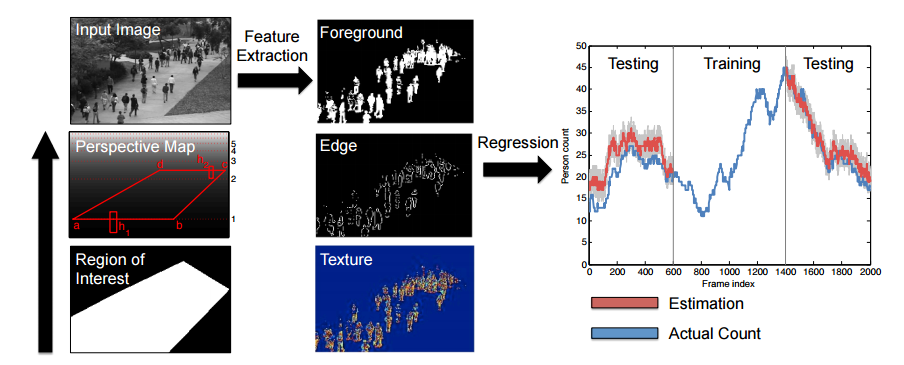
\includegraphics[scale=0.45]{22}
    				\caption{mô hình áp dụng regression: đầu tiên ta xác định khu vực quan tâm cần tính toán và tìm ra sơ đồ chuẩn hóa (normalisation map) . sau đó sẽ rút trích những đặc trưng tổng thể và huấn luyện ra mô hình hồi quy sử dụng những đặc trưng đã được chuẩn hóa.} 
    				\label{22}
  			\end{center}
\end{figure} 

	Từ những nền tảng đó cùng với những mô hình deep learning mới ra đời. Hướng tiếp cận này đã mang lại những những kết quả chính xác hơn và tốc độ cải thiện rõ rệt so với những phương pháp còn lại.  
	
\section{Kết chương}
